%==============================================================================
% Voorbeeld hogent-article: onderzoeksvoorstel bachproef
%==============================================================================

\documentclass{hogent-article}

\usepackage{lipsum} % Voor vultekst
\usepackage{bytefield} % Voor TCP Header
\usepackage{graphicx} % Voor grafiek TCP Equilibrium
\graphicspath{ {./img/} }

% Invoegen bibliografiebestand
\addbibresource{references.bib}

% Informatie over de opleiding, het vak en soort opdracht
\studyprogramme{Professionele bachelor toegepaste informatica}
\course{Bachelorproef}
\assignmenttype{Paper: Onderzoeksvoorstel}
\academicyear{2023-2024}


\title{Netwerkautomatisering aan de Universiteit Gent: Een Scriptmatige Aanpak voor Efficiënt Beheer van IP-Adressen}
\author{Stijn Coppens}
\email{stijn.coppens@student.hogent.be}

\projectrepo{https://github.com/stcoppens/Bachelorproef}

% Binnen welke specialisatierichting uit 3TI situeert dit onderzoek zich?
% Kies uit deze lijst:
%
% - Mobile \& Enterprise development
% - AI \& Data Engineering
% - Functional \& Business Analysis
% - System \& Network Administrator
% - Mainframe Expert
% - Als het onderzoek niet past binnen een van deze domeinen specifieer je deze
%   zelf
%
\specialisation{System \& Network Administrator}
% Geef hier enkele sleutelwoorden die je onderwerp beschrijven
\keywords{DNS, DHCP, IPAM, Python}

\begin{document}

\begin{abstract}
Het beheren van netwerken en het reserveren van netwerkadressen gebeurt momenteel grotendeels handmatig, wat inefficiënt is als proces, en tevens gevoelig voor menselijke fouten. 

Deze bachelorproef richt zich op het uitwerken van een innovatieve, geautomatiseerde aanpak voor het beheren van netwerken en het
toewijzen van netwerkadressen met behulp van scripts. 
Het doel van deze bachelorproef is tweeledig, namelijk (1) het creëren van een tussenlaag van scripts boven een bestaand beheerprogramma voor netwerken, en (2) het nagaan van de impact hiervan op het tijdverbruik voor het toevoegen, wijzigen en verwijderen van nieuwe IP-reserveringen in vergelijking met het huidige handmatige beheerproces. Als resultaat van de bachelorproef kan men via een webpagina die beschikbaar is binnen het bedrijfsnetwerk, mits toestemming van de netwerkbeheerder, eenvoudig netwerkadresreservaties aanmaken, wijzigen of verwijderen.
De webpagina zal de scripts, die binnen het project geschreven worden, aanroepen om de nodige gegevens op de juiste manier aan te leveren aan het beheerprogramma. 

Het verminderen van handmatig beheer van netwerkconfiguraties als resultaat van deze bachelorproef, zal leiden tot efficiëntiewinsten, tijdsbesparingen, een vereenvoudigde aanpak en minder fouten. 

% Deze bachelorproef concentreert zich op het ontwikkelen van een vernieuwende, geautomatiseerde aanpak voor netwerkbeheer en adresallocatie met behulp van scripts. Het hoofddoel is om een abstractielaag te creëren boven een bestaande tool voor netwerkbeheer. Hierbij wordt de  van een IP Address Management (IPAM)-tool aangestuurd. Deze abstractielaag maakt interactie met de IPAM-tool mogelijk via Python-scripts en wordt toegepast via eenvoudige handelingen in een gebruiksvriendelijk webportaal. 
% Netwerkconfiguraties worden momenteel grotendeels handmatig beheerd, wat inefficiënt is als proces, en tevens gevoelig is voor menselijke fouten. Het minimaliseren van handmatig beheer van netwerkconfiguraties zou leiden tot efficiëntiewinsten, tijdswinsten en verminderde complexiteit.
% Deze bachelorproef richt zich op het ontwikkelen van een innovatieve, geautomatiseerde benadering voor netwerkbeheer (en IP-adresallocatie), door middel van Python-scripts.
% Het hoofddoel is het creëren van een abstractielaag boven een bestaande netwerkbeheertool voor DNS en DHCP, waarbij de API van een IP Address Management (IPAM)-tool wordt aangestuurd. Deze abstractielaag maakt interactie met de IPAM-tool mogelijk via Python-scripts en wordt toegepast door API-aanroepen vanuit een intuïtief webportaal.

\end{abstract}
\tableofcontents

\bigskip

\section{Inleiding}%
\label{sec:inleiding}
In de snel evoluerende wereld van technologie is het doeltreffend beheren van netwerken cruciaal geworden voor het succes van organisaties. Echter, het handmatig beheren van netwerkconfiguraties, waaronder het toewijzen van specifieke netwerkadressen, blijft een tijdrovend en foutgevoelig proces.

Om deze uitdagingen aan te pakken, zijn er onder andere geautomatiseerde oplossingen voor Internet Protocol Address Management (IPAM) ontwikkeld. Een goed uitgewerkte IPAM-tool kan een grote meerwaarde bieden voor elk netwerk doordat deze o.a. een overzicht kan geven van alle IP adressen die in gebruik zijn en hoeveel IP adressen er nog beschikbaar zijn per subnet.

Dit onderzoek zal scripts voorzien die, via een webportaal en de goedkeuring van netwerkbeheerders, gebruikers zullen toelaten te communiceren met de IPAM-tool om IP reservaties te maken, wijzigen of verwijderen. Dankzij autorisatie zullen gebruikers op het webportaal enkel wijzigingen kunnen aanbrengen voor de netwerken waarvoor de gebruiker gemachtigd is dit te doen. Nadat de netwerkbeheerder die wijzigingen via hetzelfde webportaal goedkeurt, zullen de scripts in werking treden waarbij de nodige aanpassingen gemaakt worden binnen de gebruikte IPAM-tool.

Het automatisch beheren van IPAM via scripts beoogt niet alleen de efficiëntie van het netwerkbeheer te verhogen, maar ook tijdsbesparingen te realiseren en een meer gestroomlijnde aanpak te bieden. Deze tijdsbesparingen zijn de focus van het onderzoek, waarbij we de volgende onderzoeksvraag trachten te beantwoorden: Hoe beïnvloedt de implementatie van \\geautomatiseerde scripts het tijdverbruik voor het toevoegen, wijzigen en verwijderen van nieuwe IP-reserveringen in vergelijking met het huidige handmatige beheerproces?

\subsection{Probleemstelling}
\label{sec:probleemstelling}
Deze bachelorproef zal uitgevoerd worden bij Universiteit Gent (UGent), directie ICT. Momenteel werkt UGent met scripts die op basis van zogenaamde \textit{subnetbestanden} de nodige acties doen om het netwerk te beheren. 

Deze ongecrypteerde subnetbestanden stellen elk een subnetwerk (een aantal opeenvolgende netwerkadressen) voor en beschrijven cruciale informatie zoals belangrijke naamservers, welk \textit{Virtual Local Area Network (VLAN)} nummer, gateway, etc. Hiernaast bevatten deze zowel alle beschikbare als gereserveerde netwerkadressen met daarbij eventueel enkele regels voor domeinnamen en beveiliging.

Voor elke netwerkadresreservatie die moet gebeuren, vullen geautoriseerde gebruikers via een webportaal alle nodige info in.
Nadat ze deze inzenden stuurt het webportaal een mail naar de groep mailbox van de netwerkbeheerders.
In deze mail zitten dan alle nodige commando's en teksten om de gevraagde wijzigingen aan te brengen aan de relevante subnetbestanden. In sommige gevallen dient de netwerkbeheerder eerst zelf nog uit te zoeken welk subnetbestand nodig is op basis van de documentatie en opzoekwerk. Indien de aanvrager van de reservatie dit heeft meegegeven in een veld voorzien voor commentaar, moet de netwerkbeheerder de eventuele domeinnaam- of beveiligingsregels handmatig toevoegen aan de reservatie.

Het overzicht van de beschikbare subnetwerken is beschreven in een interne wikipediapagina met daarbij de beschrijving van elk subnetwerk. Deze huidige aanpak brengt meerdere uitdagingen met zich mee:
\begin{itemize}
    \item \textbf{Tijd}: Het manueel onderhouden van de \\scripts, subnetbestanden, netwerkadresreservaties (maken en opkuisen) kan veel tijd vragen. Alle mails met IP registraties moeten elk afzonderlijk bekeken en verwerkt worden.
    \item \textbf{Schaalbaarheid}: Doordat elke wijziging het bestaande bestand overschrijft en er dus \\geen historische data is kan men moeilijk trends herkennen. Ook wikipediapagina's moet men manueel bijwerken bij grote wijzigingen in de structuur.
    \item \textbf{Consistentie}: De huidige aanpak vraagt \\meerdere manuele acties, waardoor die vatbaar is voor menselijke fouten of vergissingen. Ook het manueel opzoeken van de relevante subnetbestanden als de aanvrager niet weet in welk subnet de aanvraag terecht moet komen, kan leiden tot registraties in verkeerde subnetten.  
    \item \textbf{Beveiliging}: Zoals beschreven door \textcite{Liao2020} is een van de eerste stappen in een cybersecurity aanval het verzamelen van netwerk informatie via netwerk scan tools zoals Nmap. Het bewaren van alle IP registraties van het volledige domein centraal in cleartext bestanden, zoals nu het geval is, is dan ook een schat aan informatie voor elke individu met al dan niet slechte bedoelingen.
\end{itemize}

UGent is momenteel stappen aan het ondernemen voor het implementeren van \textit{Efficiënt IP (EIP)}, een IPAM-softwarepakket. Dankzij deze implementatie is de verwachting dat de hierboven beschreven indicatoren zullen verbeteren. Om de onderzoeksvraag te beantwoorden zullen er metingen gedaan worden betreffende tijdverbruik. Hierbij zal de huidige manier van werken in tijdsgebruik vergeleken worden met die na de implementatie van het webportaal.

\subsection{Doelstelling}
\label{sec:doelstelling}
Deze bachelorproef zal een abstractielaag maken boven EIP waarbij scripts via de \textit{Application Programming Interface (API)} van EIP \\commando's zullen uitvoeren op EIP.
Door de omvang van het EIP-project is het binnen de voorziene tijd van de bachelorproef niet haalbaar om UGent volledig over te zetten op de werking van EIP. Aangezien dit kritische componenten zijn, zal alles eerst uitvoerig getest worden waarbij elke stap in de migratie naar EIP weloverwogen is.

Daarom stel ik als doel om een eerste versie op te leveren van een webportaal waarop men reeds één of meerdere netwerkadresreservaties kan aanmaken, wijzigen of verwijderen. Aangezien elk subnet specifiek is voor bepaalde verdiepingen, gebouwen en/of vakgroepen, en elke medewerker binnen UGent tot een specifieke vakgroep behoort, zullen we deze informatie gebruiken om te bepalen voor welke relevante subnetten de aanvrager wijzigingen kan aanvragen. Deze aanvragen komen in een duidelijk overzicht terecht waar de netwerkbeheerders al dan niet \\openstaande reservaties kunnen wijzigen, goedkeuren of weigeren. Na goedkeuring worden de scripts gebruikt om de reservaties toe te passen in EIP.

Dit project geeft een antwoord op de vraag: Hoe kunnen netwerkbeheerders hun werk vereenvoudigen door het gebruik van scripts?
Het beoogde resultaat is:
\begin{itemize}
    \item Het vereenvoudigen van veelvoorkomende taken, zoals het reserveren van internetadressen.
    \item Tijd besparen door het vermijden van handmatige handelingen.
    \item Efficiënter werken door menselijke fouten te voorkomen.
    \item De gebruiksvriendelijkheid verbeteren.
\end{itemize}

Deze verbeteringen zullen helpen bij het optimaliseren van de netwerkinfrastructuur.

% In de hedendaagse technologische omgeving is netwerkbeheer van cruciaal belang voor de \\soepele werking van bedrijfsinfrastructuren. Traditioneel vereist het beheren van \\netwerkconfiguraties, met name \textit{Domain Name System (DNS)} en \textit{Dynamic Host Configuration Protocol (DHCP)}, een grote mate van handmatige inspanning. Dat kan leiden tot inefficiëntie en menselijke fouten. Om dit op te lossen bestaan er meerdere \textit{Internet Protocol Address Management (IPAM)} softwarepakketten om de taken van netwerkbeheerders te automatiseren. 

% Het hoofddoel van deze bachelorproef is het ontwikkelen van een praktische oplossing voor netwerkbeheer door middel van python-scripts, waardoor een abstractielaag bovenop een IPAM-tool ontstaat. Deze laag zal de interactie mogelijk maken tussen een webportaal waar gebruikers veel voorkomende acties kunnen aanvragen die dan mits goedkeuring van de netwerkberheerder de IPAM kunnen aansturen.

% Dit onderzoek zal een antwoord bieden op de vraag hoe je via python scripts een abstractielaag kan voorzien om via een webapplicatie veelgebruikte acties door te sturen naar de \textit{Application Programming Interface (API)} van een IPAM-tool. 

% Uit dit project worden volgende voordelen verwacht:
% \begin{itemize}
%    \item Verminderde complexiteit voor \\veelgebruikte acties zoals het reserveren van IP-adressen.
%    \item Tijdwinst door het uitsluiten van handmatig beheer.
%    \item Efficiëntie door het vermijden van menselijke fouten.
%    \item Verbetering van gebruiksvriendelijkheid
%\end{itemize}
% Deze voordelen zullen bijdragen aan een gestroomlijnde netwerkinfrastructuur.

% Dit onderzoek zal een eerste versie van het webportaal maken waarop gebruikers een \textit{Internet Protocol (IP)} reservatie kunnen aanvragen, wijzigen of verwijderen, nadat deze actie is goedgekeurd door een netwerkbeheerder zal deze dan uitgevoegd worden door de IPAM.

% TODO: (fase 1) introduceer je gekozen onderwerp, formuleer de onderzoeksvraag en deelvragen. Wat is de doelstelling (is die S.M.A.R.T.?), wat zal het resultaat zijn van het onderzoek (een Proof-of-Concept, een prototype, een advies, ...)? Waarom is het nuttig om dit onderwerp te onderzoeken?

\section{Literatuurstudie}
\label{sec:begrippen}
Internet Protocol (IP) is het fundament van elk gestructureerd, goed functionerend en veilig netwerk. Het geeft de mogelijkheid efficiënt gegevens te routeren, netwerken te verdelen in meer beheersbare eenheden, toegang te beperken tot gevoelige data of systemen, services te identificeren en het oplossen van netwerkproblemen \autocite{Postel1981}. Dit hoofdstuk legt uit wat \textit{Domain Name System (DNS)} en \textit{Dynamic Host Configuration Protocol (DHCP)} is, waarom IPAM helpt bij het beheren van IP netwerken en waarom HTTP nodig is om te communiceren met EIP. 

\subsection{DNS}
\textcite{Mockapetris1987} schrijft dat DNS een systeem is dat \textit{resource records} gebruikt om onder andere vertalingen te voorzien tussen domeinnamen en IP-adressen. Als voorbeeld kan je via de browser naar google surfen via het IP-adres \textit{142.251.36.35} of via domeinnaam\\ \textit{www.google.be}.
\\ \\
Zoals beschreven door \textcite{Mockapetris1987} voorziet DNS meerdere types resource records die netwerkbeheerders kunnen meegeven: 
\begin{itemize}
    \item \textbf{A}: Dit resource record beschrijft een host adres. 
    Vb. \textit{”server1.voorbeeld.com. IN A \\192.168.1.1”} maakt de vertaling zodat het toestel met de domeinnaam \textit{server1.voorbeeld.\\com} bereikbaar is zowel via het IP-adres\\ \textit{192.168.1.1} als via de domeinnaam. 
    \item \textbf{CNAME}: Dit resource record beschrijft de canonieke naam van een host, het wordt gebruikt om een alias of subdomein naar het hoofddomein door te verwijzen. Vb.\\ \textit{"www.voorbeeld.com. IN CNAME \\server1.voorbeeld.com"} zorgt dat server1 ook bereikbaar is via "\textit{www.voorbeeld.com}".
    \item \textbf{MX}: Dit resource record is een \textit{mail exchange} record en wordt gebruikt om aan te geven welke mailservers verantwoordelijk zijn voor het ontvangen van mails binnen een domein. vb. \textit{"voorbeeld.com. IN MX 10 mailserver.voorbeeld.com"} geeft de DNS server mee welke server de mailserver is.
    \item \textbf{NS}: Dit resource record is een \textit{name server} record, het beschrijft welke DNS-servers verantwoordelijk zijn voor het beheren van DNS-informatie voor een domein. Vb. \textit{"voorbeeld.com. IN NS dns1.voorbeeld.com"} verwijst naar \textit{dns1} als DNS-server voor het domein “\textit{voorbeeld.com}”.
    \item \textbf{PTR}: Dit resource record is een \textit{Pointer} record, het wordt gebruikt om via IP een vertaling te vragen aan de DNS-server in plaats van via de naam.
    \item \textbf{SOA}: Dit resource record is een \textit{Start of Authority} record die belangrijke informatie bevat over de zone, zoals welke de primaire DNS-server, contactpersonen, etc. zijn.
\end{itemize}

\subsection{DHCP}
Dit protocol voorziet een framework voor het doorgeven van configuratie-informatie naar \\hosts (lees: computers) op het netwerk . Zo kan een computer bijvoorbeeld een IP-adres ontvangen waarmee die kan communiceren binnen het netwerk waarop die is aangesloten \autocite{Droms1997}.

IP-netwerken worden door netwerkbeheerders op een logische manier opgesplitst in subnetwerken. Hierbij worden de beschikbare IP-adressen verdeeld in subnetwerken (subnet). Toestellen binnen subnet A zullen elkaar kunnen bereiken terwijl een toestel in een subnet B zonder de nodige routering geen verbinding zal kunnen maken met de toestellen in subnet A.

Voor DHCP zullen netwerkbeheerders subnets (of pools van IP-adressen) aanbieden aan de \\DHCP-server. Die zal gebruik maken van deze pools door (onder andere) IP-adressen uit te delen aan toestellen die verbinden op het netwerk en daarbij de DHCP-server laten weten dat ze nog geen IP-adres hebben.

\textcite{Droms1997} schrijft dat DHCP drie mechanismes gebruikt voor het uitdelen van IP-adressen:
\begin{itemize}
    \item \textbf{Automatisch}: Permanent toewijzen van een IP-adres.
    \item \textbf{Dynamisch}: IP-adres voor een bepaalde tijd toewijzen.
    \item \textbf{Manueel}: Een (door de netwerkbeheerder) vooraf bepaald IP-adres toewijzen, in vakjargon noemt met dit een IP-reservatie.
\end{itemize}

\subsection{IPAM}
Naast de vele uitdagingen die zowel DNS als DHCP met zich meebrengen, is het beheren van de vele DNS records, IP-adres ranges en de vaak vele IP-reservaties zeker iets waar een netwerkbeheerder over moet waken. 
Een mogelijke oplossing hiervoor is het gebruiken van IP Address Management (IPAM) via softwarepakketten die IPAM aanbieden.
IPAM laat toe IP-adressen efficiënt te beheren in een netwerk, het leidt tot een gestructureerde aanpak waardoor conflicten tussen subnetten worden vermeden. Het geeft een compleet overzicht van het netwerk met percentages van hoeveel adressen beschikbaar en in gebruik zijn. IPAM geeft eveneens de mogelijkheid om de historiek bij te houden waardoor het van pas komt voor schaalbaarheid en beveiliging van het netwerk \autocite{Rooney2020}.

\subsection{HTTP/HTTPS}
Om communicatie met de API van EIP mogelijk te maken wordt er gebruik gemaakt van \textit{Hypertext Transfer Protocol (HTTP)}. Dit is een client-serverprotocol die communicatie mogelijk maakt op het Internet. Zoals beschreven door \textcite{Fielding2014} maakt HTTP gebruik van \textit{Uniform Resource Identifiers (URI's)} om unieke web-resources te identificeren en biedt het verschillende methoden \textit{(GET, POST, PUT, DELETE)} waarmee clients acties kunnen uitvoeren op serverresources. HTTP is \textit{stateless}, elke aanvraag is onafhankelijk, en statuscodes zoals "200 OK"\ en \textit{headers} worden gebruikt om de resultaten en aanvullende informatie van serververzoeken aan te geven, waardoor een gestandaardiseerde communicatie tussen clients en servers mogelijk is.
Om deze informatieoverdracht te beveiligen, \\wordt \textit{Hypertext Transfer Protocol Secure (HTTPS)} gebruikt. HTTPS bouwt voort op HTTP, maar voegt een extra beveiligingslaag toe door middel van \textit{Secure Sockets Layer (SSL)/Transport Layer Security (TLS)}-encryptie, \\waardoor de uitwisseling van gegevens tussen client en server wordt versleuteld. Hierdoor worden alle IP-registraties en andere gegevens beter beschermd tegen potentiële aanvallen.

\section{Methodologie}
\label{sec:methodologie}
In dit hoofdstuk wordt beschreven hoe lang en hoe de nodige metrics voor de onderzoeksvraag worden opgemeten, welke software het project gebruikt, hoe deze worden toegepast, en welke fases het project zal doorlopen.

\subsection{Software}
Alle scripts worden geschreven in \textbf{Visual studio code} in de programmeertaal \textbf{Python}.
Om de HTTP methodes naar de API van EIP te testen, wordt er gebruik gemaakt van \textbf{Postman}.
\begin{itemize}
    \item \textbf{Visual Studio Code}: Vanwege de ondersteuning voor meerdere programmeer- en scripttalen, geïntegreerde Git-ondersteuning, debug- en extensie mogelijkheden wordt gekozen om alle scripts in Visual Studio Code te schrijven.
    \item \textbf{Python}: \textcite{VanRossum2011} beschrijven Python als een eenvoudige, doch krachtige programmeertaal. De beschikbaarheid van Python-pakketten zoals ’requests’ maakt het mogelijk om efficiënt gegevens door te sturen naar API’s zoals die van EIP. Als interpretatieve taal biedt Python snelle ontwikkeling zonder de noodzaak van compilatie. Python is ook uitbreidbaar, waardoor het eenvoudig is om nieuwe functies toe te voegen. Kortom, Python, met zijn netwerkbibliotheken, vormt een ideale keuze voor dit onderzoeksproject \autocite{VanRossum2011}.
    \item \textbf{Postman}: Dit programma geeft de mogelijkheid alle HTTP-verzoeken manueel te maken, versturen en ontvangen. Hierbij is het mogelijk om alle onderdelen van het verzoek te manipuleren en na te gaan wat als resultaat verwacht kan worden bij het uitsturen van bepaalde verzoeken naar de API.
\end{itemize}

\subsection{Methodiek scripts}
Voordat een script wordt geschreven, worden eerst gerichte testen gedaan waarbij commando's met parameters naar de API van EIP worden verzonden. Hierbij wordt er zowel naar de resultaten van de API gekeken als naar wat er op EIP zelf gebeurt via de webpagina. Eens deze testen voor een commando afgelopen zijn, wordt er pas overgegaan tot het schrijven van het Python-script. Hierbij worden telkens de parameters binnen elk script opgezet volgens de voorwaarden van de API.

\subsection{Fase 1. Pre-analyse}
In de eerste fase van de bachelorproef worden er dagelijks metingen gedaan om na te gaan hoeveel tijd een netwerkbeheerder van UGent gebruikt om IP reservaties aan te maken, te wijzigen en/of te verwijderen. Hierbij wordt voor elk type actie de tijd afzonderlijk gemeten en beschreven in een spreadsheet die als bijlage aan het onderzoek wordt toegevoegd.

\subsection{Fase 2. Literatuurstudie}
Voor deze tweede fase worden veertien dagen uitgetrokken. In deze fase wordt gezocht naar documentatie en literatuur van gelijkaardige projecten waarbij een webpagina met formulieren en logins gebruiken om scripts aan te roepen. Daarnaast wordt er ook uitgebreid aandacht gegeven aan de literatuur van Efficiënt IP zelf om na te gaan welke eisen deze stelt voor het aanmaken, wijzigen en verwijderen van IP-adressen.
Op het einde van deze fase zal er een verslag geschreven worden met alle belangrijke punten die zijn meegenomen uit de literatuur.

\subsection{Fase 3. Scripts schrijven}
Binnen de derde fase wordt het grootste stuk van de Python-scripts geschreven. Deze fase voorziet telkens één week om een script te schrijven en daarop aansluitend één week om het geschreven script te testen en te troubleshooten. De drie scripts zijn:
\begin{itemize}
    \item Maken van een IP reservatie
    \item Wijzigen van een bestaande IP reservatie
    \item Verwijderen van een bestaande IP reservatie
\end{itemize}

\subsection{Fase 4. Webpagina schrijven}
Het schrijven van de webpagina begint halverwege fase twee aangezien deze nauw op elkaar aansluiten.
Voor het schrijven van de hoofdpagina van waar de drie scripts kunnen worden aangeroepen, worden drie weken voorzien. Hierna zijn er nog drie weken voorzien voor het schrijven van de netwerkbeheerderspagina. Op deze pagina kan de netwerkbeheerder de gevraagde wijzigingen nakijken, aanpassen en goed- of afkeuren. 

\subsection{Fase 5. Post-analyse}
Tijdens deze laatste fase worden er opnieuw metingen gedaan om na te gaan hoeveel tijd de netwerkbeheerders van UGent nodig hebben voor elke afzonderlijke registratie. Ook in deze fase zullen de metingen in een spreadsheet komen om de nodige vergelijkingen te maken met de data uit de eerste fase van de bachelorproef.

\subsection{Gantt stappenplan}
Een overzicht van alle fases worden weergegeven in dit Gantt stappenplan
\begin{figure}[h!]
    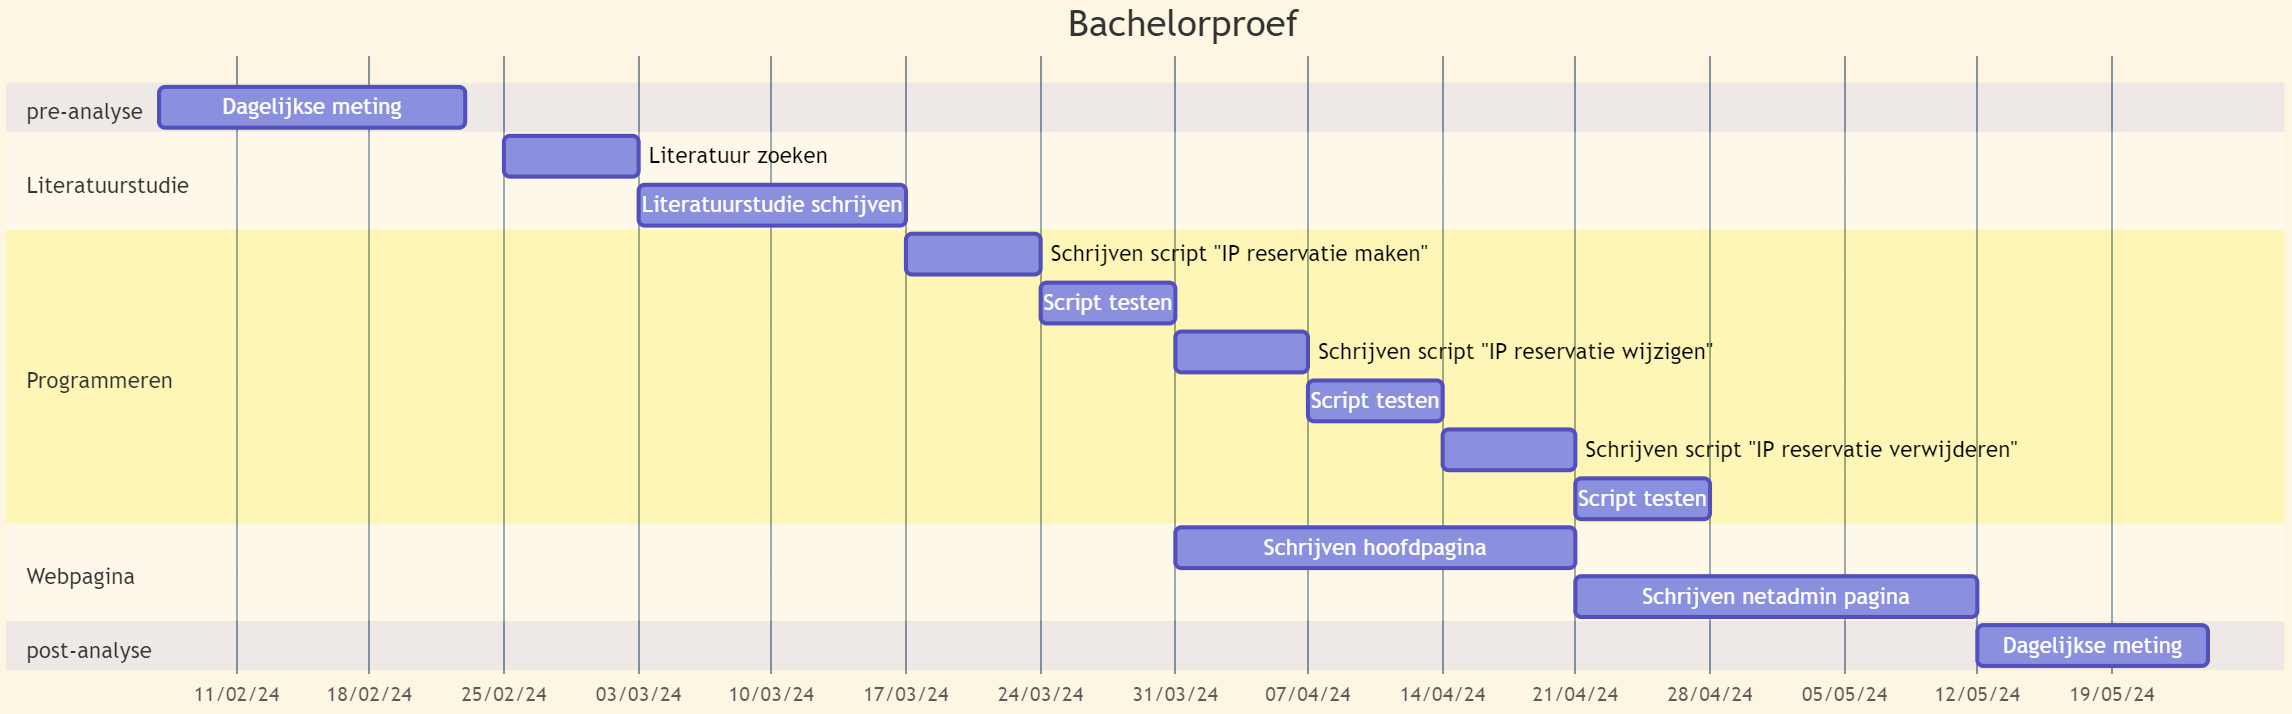
\includegraphics[scale=0.21]{Gantt}
    \caption{Gantt Stappenplan}
    \label{Gantt Stappenplan}
\end{figure}

% Refereren naar de literatuur kan met:
% \autocite{BIBTEXKEY} -> (Auteur, jaartal)
% \textcite{BIBTEXKEY} -> Auteur (jaartal)
% Voorbeeld van een referentie waar de auteursnaam geen onderdeel van de zin is~\autocite{Moore2002}.

\section{Verwachte resultaten}
\label{sec:verwachte-resultaten}
% TODO: (fase 6) beschrijf wat je verwacht uit je onderzoek en waarom (bv. volgens je literatuuronderzoek is softwarepakket A het meest gebruikte en denk je dat het voor deze casus ook het meest geschikt zal zijn). Natuurlijk kan je niet in de toekomst kijken en mag je geen alternatieve mogelijkheden uitsluiten. In de praktijk gebeurt het ook vaak dat een onderzoek tot verrassende resultaten leidt, dat maakt het proces nog interessanter!
De verwachte resultaten omvatten een succesvolle eerste implementatie van een webportaal waarop men reeds één of meerdere netwerkadresreservaties kan aanmaken, wijzigen of verwijderen. Deze eerste versie van het intuïtieve webportaal zou een verbeterde gebruikerservaring moeten bieden door middel van geoptimaliseerde API-aanroepen. Verder zou de automatisering van netwerkconfiguraties, \\met name IP-adresallocatie, moeten leiden tot verminderde complexiteit, verbeterde efficiëntie en algemene gebruiksvriendelijkheid in het netwerkbeheerproces. Dit zal een belangrijke stap zijn om na het project op voort te bouwen om uiteindelijk een product op te leveren.


\section{Verwachte conclusie}
\label{sec:discussie-conclusie}
Dankzij het implementeren van deze webpagina met de onderliggende scripts, kunnen medewerkers van Universiteit Gent eenvoudig, consistent, en snel IP-reservaties maken, wijzigen en verwijderen. De netwerkbeheerders kunnen al deze wijzigingen dan op hun eigen webpagina controleren, aanpassen en beoordelen.
Na dit onderzoek zullen er nog voldoende mogelijkheden zijn om de webpagina aan te vullen met extra functies, in die mate dat netwerkbeheerders zelf geen wijzigingen meer dienen te maken binnen de IPAM tool zelf.

%------------------------------------------------------------------------------
% Referentielijst
%------------------------------------------------------------------------------
% TODO: (fase 4) de gerefereerde werken moeten in BibTeX-bestand
% bibliografie.bib voorkomen. Gebruik JabRef om je bibliografie bij te
% houden.

\printbibliography[heading=bibintoc]

\end{document}